\documentclass[10pt,a4paper]{report}
\usepackage[utf8]{inputenc}
\usepackage{amsmath}
\usepackage{amsfonts}
\usepackage{amssymb}
\usepackage{float}
\usepackage{graphicx}
\graphicspath{{./images/}}
\usepackage{mathtools}
\DeclarePairedDelimiter\abs{\lvert}{\rvert}
\usepackage[left=3.00cm, right=3.00cm, top=3.00cm, bottom=3.00cm]{geometry}
\author{Del Prete Giovanni, Ghilardi Nicola, Polver Marco}
\title{BookSales UniBG: iterazione 0}
\begin{document}
	
	\maketitle
	\tableofcontents
	
	\section{Requisiti e scelte progettuali}
	\subsection{Obiettivi}
	\textit{BookSales UniBG} è un'applicazione web ideata con l'idea di favorire e migliorare i processi di compravendita di libri universitari all'interno dell'Università degli Studi di Bergamo. 
	\\
	Attualmente per la vendita di libri gli studenti utilizzano mezzi quali le bacheche distribuite nelle diverse sedi, gruppi sui social network e siti web di annunci oppure sfruttano le proprie conoscenze personali. Tutti questi mezzi risultano avere problemi di inefficacia dovuti alla scarsa visibilità dei libri messi in vendita oppure alla natura troppo "general purpose" dei servizi online utilizzati.\\
	\textit{BookSales UniBG} si propone di fornire un mezzo per la vendita di libri universitari che sia in grado di:
	\begin{enumerate}
		\item Facilitare l'inserimento di un'inserzione da parte di un venditore.
		\item Mostrare ai potenziali acquirenti tutti quei libri che con maggior probabilità potrebbero far parte dei loro interessi.
		\item Favorire compravendite soddisfacenti.
		\item Impedire la compravendita di appunti o libri fotocopiati.
		\item Garantire l'accesso al servizio da qualsiasi dispositivo connesso in rete.
	\end{enumerate}

	\subsection{Requisiti funzionali}
	Per la comprensione dei requisiti è necessario chiarire il significato dato ai seguenti termini:
	\begin{itemize}
		\item \textit{Libro}: si intende uno specifico libro in vendita, con relativa inserzione.
		\item \textit{Titolo}: si intende un elaborato generico, non una sua realizzazione fisica.
	\end{itemize}
	Esempio: "Fondamenti di meccanica per l'ingegneria" è un titolo, mentre per libro si potrebbe intendere una sua qualsiasi realizzazione fisica messa in vendita da un utente. \\
	
	\begin{tabular}{cp{3cm}p{9cm}p{1cm}}
		Codice requisito&Nome&Descrizione\\ \hline
		AC1&Registrazione nuovo studente&Registrazione e verifica dei dati di un nuovo studente che intende usufruire del servizio. I dati da fornire obbligatoriamente durante la registrazione dovranno essere i seguenti:
		\begin{itemize}
			\item Username desiderato
			\item Nome e cognome
			\item Mail universitaria UniBG
			\item Corso di laurea e anno di corso
			\item Password
		\end{itemize}
		A richiesta di registrazione effettuata, il sistema deve verificare che nessuno studente si sia già registrato con l'indirizzo email universitario e lo username inseriti e verificare che la password sia sufficientemente sicura, ovvero che:
		\begin{itemize}
			\item Sia composta da almeno 8 caratteri.
			\item Non sia totalmente numerica.
			\item Non sia troppo simile ai dettagli personali forniti.
			\item Non sia una password banale (es. 00000000)
		\end{itemize}\\ \hline
		AC2&Accesso studente&Accesso al servizio da parte di uno studente precedentemente registrato tramite inserimento di username e password.\\ \hline
		AC3&Logout studente&Logout da parte di uno studente che ha precedentemente effettuato l'accesso al servizio.\\ \hline
	\end{tabular}

	\begin{tabular}{cp{3cm}p{9cm}p{1cm}}
		Codice requisito&Nome&Descrizione\\ \hline
		RI1&Ricerca libro&Ricerca da parte di uno studente di un libro di testo in vendita con filtraggio basato su:
		\begin{itemize}
			\item Titolo
			\item Prezzo
			\item Condizioni del libro:
			\begin{itemize}
				\item Classe A: libro intatto senza sottolineature o appunti.
				\item Classe B: libro intatto con sottolineature e appunti.
				\item Classe C: libro con piccoli segni d'usura, sottolineature e appunti.
				\item Classe D: libro con pagine stropicciate o rovinate, pieghe della copertina, sottolineature e appunti.
			\end{itemize}
			
		\end{itemize}\\ \hline
		RI2&Visualizzazione libri consigliati&Visualizzazione nella pagina "Suggested ads" di libri potenzialmente interessanti sulla base di:
		\begin{itemize}
			\item Interesse mostrato esplicitamente dallo studente tramite inserimento di uno specifico libro nella lista "Wishlist" (\textit{RI3}) o tramite inserimento di un titolo nella lista "Titoli d'interesse" (\textit{RI4}).
			\item Interesse mostrato da studenti aventi caratteristiche simili: a tal fine un metodo di clusering deve essere definito.
		\end{itemize}\\ \hline
		RI3&Inserimento libro in lista "Wishlist"&Inserimento da parte di uno studente di uno specifico libro in vendita (non un titolo) nella lista "Wishlist", la quale contiene riferimenti agli annunci che lo studente intende seguire.\\ \hline
		RI4&Inserimento titolo in lista "Titoli d'interesse"&Inserimento da parte di uno studente di un titolo nella lista "Titoli d'interesse", la quale permette allo studente di seguire facilmente tutti gli annunci relativi a libri legati a determinati titoli.\\ \hline
	\end{tabular}

	\begin{tabular}{cp{3cm}p{9cm}p{1cm}}
		Codice requisito&Nome&Descrizione\\ \hline
		I1&Inserimento annuncio&Inserimento da parte di uno studente di un annuncio per la vendita di un libro. L'inserzione deve contenere le seguenti informazioni mandatorie:
		\begin{enumerate}
			\item Titolo: deve essere selezionato da una lista di titoli già presenti nel sistema. In caso di assenza si richiede allo studente di inserire le informazioni del libro nel sistema affinché queste siano disponibili in futuro (\textit{I2}).
			\item Almeno una foto.
			\item Prezzo.
			\item Descrizione.	
			\item Condizioni del libro seguendo le indicazioni formalizzate in (\textit{R1}).
		\end{enumerate}
		Una volta confermata da parte dell'utente la richiesta di inserimento dell'inserzione, il sistema verifica che siano rispettate le seguenti condizioni:
		\begin{itemize}
			\item Lo studente non deve aver proposto un'inserzione relativa allo stesso libro negli ultimi 7 giorni.
			\item Il commento al libro non deve contenere parole scurrili.
		\end{itemize}
		Se l'annuncio rispetta le condizioni di cui sopra, il sistema lo inserisce nel database e conferma l'accettazione della richiesta allo studente. In caso di rifiuto dell'annuncio, il sistema richiederà allo studente di attendere in caso di mancato rispetto del primo punto o di modificare la descrizione in caso di mancato rispetto del secondo punto.\\ \hline
		I2&Modifica annuncio&Modifica del contenuto di un annuncio da parte dello studente a cui appartiene.\\ \hline
	\end{tabular}
	\newpage
	\begin{tabular}{cp{3cm}p{9cm}p{1cm}}
		Codice requisito&Nome&Descrizione\\ \hline
		I3&Inserimento di un nuovo titolo&Inserimento da parte di uno studente di un titolo assente dal sistema. Le informazioni da fornire sono le seguenti:
		\begin{itemize}
			\item Titolo
			\item Autore/i
			\item ISBN
			\item Categoria (informatica, meccanica, letteratura latina, economia aziendale, ...)
		\end{itemize}
		Il sistema verifica che nessun altro titolo con il medesimo ISBN sia stato inserito in precedenza e, se ciò non è avvenuto, inserisce il titolo nel database e crea automaticamente una pagina del titolo contenente le informazioni fornite.\\ \hline
		U1&Ricerca studente&Ricerca di studenti da parte di un utente con filtraggio basato su:
		\begin{itemize}
			\item Username
			\item Corso di laurea
			\item Anno di corso
		\end{itemize}\\ \hline
		U2&Accesso pagina studente&Accesso alla pagina personale di un altro studente, la quale deve contenere informazioni quali:
		\begin{itemize}
			\item Username
			\item Nome e cognome
			\item Contatti (numero di telefono, mail, pagina Facebook, ...)
			\item Numero di libri venduti
			\item Numero di libri acquistati
			\item Voto medio recensioni ricevute
			\item Numero di recensioni effettuate (sia nel ruolo di venditore che in quello di acquirente)
			\item Recensioni ricevute in qualità di venditore
			\item Recensioni ricevute in qualità di acquirente
			\item Libri in vendita
		\end{itemize}\\ \hline
		U2.1&Accesso pagina personale studente&Accesso alla propria pagina personale da parte di uno studente. La pagina deve fornire le medesime informazioni fornite in \textit{U2}, ma deve risultare sempre accessibile con un solo click, qualunque sia la pagina del sito web aperta nell'istante corrente.\\ \hline
		U3&Modifica informazioni personali studente&Modifica da parte di uno studente delle informazioni mostrate nella propria pagina personale.\\ \hline
	\end{tabular}
	\newpage
	
	\begin{tabular}{cp{3cm}p{9cm}p{1cm}}
		Codice requisito&Nome&Descrizione\\ \hline
		T1&Ricerca pagina titolo&Ricerca da parte dell'utente della pagina relativa ad un titolo. La pagina deve contenere, se presenti, informazioni riguardanti gli argomenti trattati dal libro e le recensioni degli utenti sull'utilità del libro ai fini dell'esame.\\ \hline
		T2&Modifica pagina titolo&Modifica della pagina contenente le informazioni di un titolo da parte di un utente. Le informazioni che possono essere aggiunte sono le seguenti:
		\begin{itemize}
			\item Immagine della copertina
			\item Argomenti trattati
		\end{itemize}\\ \hline
		V1&Vendita libro&Comunicazione da parte del venditore dell'avvenuta cessione del libro legato ad una specifica inserzione. Il venditore deve fornire come informazione il nome utente dell'acquirente. Una volta avvenuto questo, il sistema deve inviare una email all'acquirente in cui viene chiesto di confermare l'acquisto del libro (\textit{V2}).\\ \hline
		V2&Richiesta conferma acquisto&Il sistema invia all'utente citato dal venditore come acquirente una email per richiedere la conferma dell'acquisto. L'email deve contenere un link ad una pagina in cui l'acquirente potrà confermare o negare l'acquisto (\textit{V3}).\\ \hline
		V3&Conferma acquisto&Conferma o negazione dell'acquisto di un libro da parte dell'utente che è stato indicato dal venditore quale l'acquirente del libro oggetto della cessione. La pagina deve contenere un riassunto dell'inserzione in questione (foto principale, titolo, nome utente del venditore e prime 5 righe della descrizione).
		In caso di conferma dell'acquisto:
		\begin{itemize}
			\item l'acquirente verrà invitato a recensire il venditore;
			\item il libro verrà rimosso dall'elenco dei libri in vendita e da tutte le liste personali ("wishlist" e "titoli d'interesse") in cui è presente;
			\item verranno aggiornati i dati relativi al numero di libri venduti e acquistati dei due utenti coinvolti;
			\item il sistema invierà una email al venditore per comunicargli l'avvenuta conferma dell'acquisto ed invitarlo a recensire l'acquirente.
		\end{itemize}
		In caso di negazione dell'acquisto, il venditore deve essere notificato via email dell'avvenuto ed invitato a rieffettuare la procedura \textit{V1} selezionando un utente differente. \\ \hline
	\end{tabular}

	\begin{tabular}{cp{3cm}p{9cm}p{1cm}}
		Codice requisito&Nome&Descrizione\\ \hline
		RE1&Recensione venditore&Inserimento da parte di un utente acquirente di una recensione del venditore di uno specifico libro. Questo dovrà risultare possibile soltanto dopo la conferma dell'acquisto di un libro. La recensione dovrà contenere un valore intero compreso tra 0 e 5 (indicato tramite stelle) ed un commento.\\ \hline
		RE2&Recensione acquirente&Inserimento da parte di un utente venditore di una recensione dell'acquirente di uno specifico libro. Questo dovrà risultare possibile soltanto dopo la conferma dell'acquisto di un libro. La recensione dovrà contenere un valore intero compreso tra 0 e 5 (indicato tramite stelle) ed un commento.\\ \hline
		RE3&Recensione titolo&Inserimento da parte di un utente qualsiasi di una recensione di un qualsiasi titolo. La recensione dovrà contenere un valore intero compreso tra 0 e 5 (indicato tramite stelle) ed un commento.\\ \hline
	\end{tabular}
	
	\section{Casi d'uso}
	Di seguito sono riportati i diagrammi dei casi d'uso.
	
	\begin{figure}[H]
		\centering
		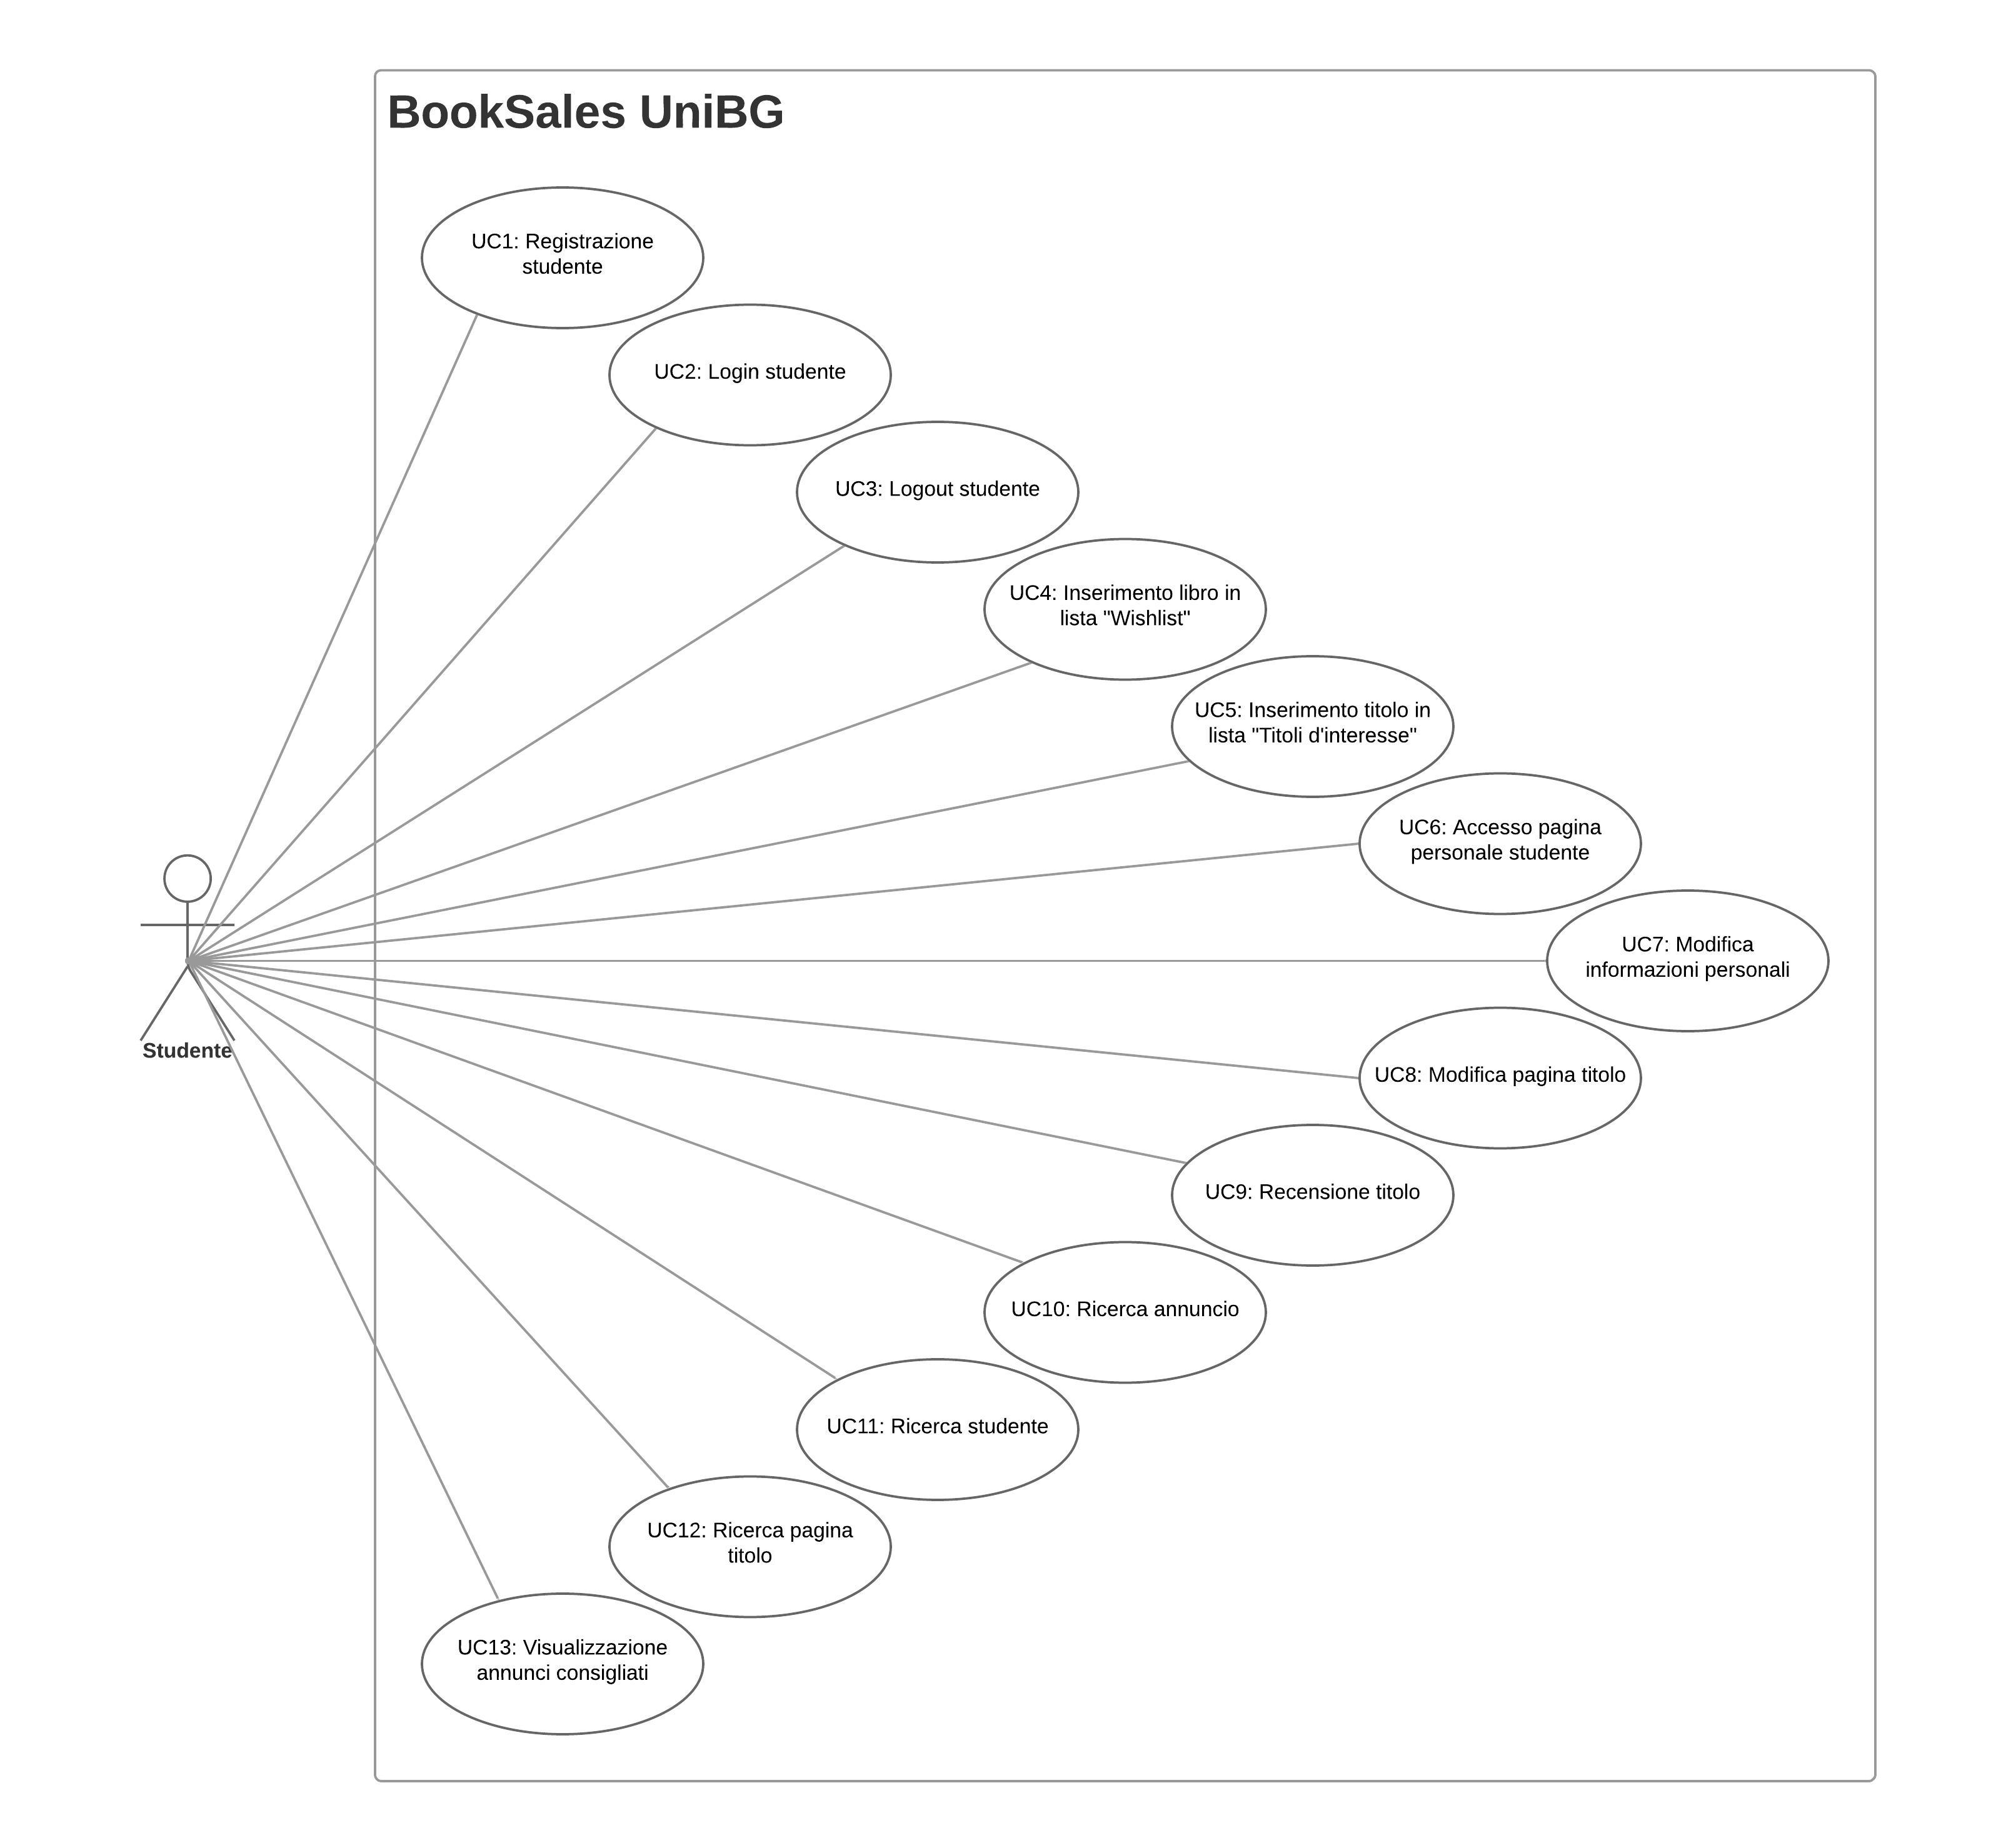
\includegraphics[height=12cm, width=17cm, keepaspectratio]{g_uc}
		\caption{Casi d'uso per utente generico e amministratore}
	\end{figure}

	\begin{figure}[H]
		\centering
		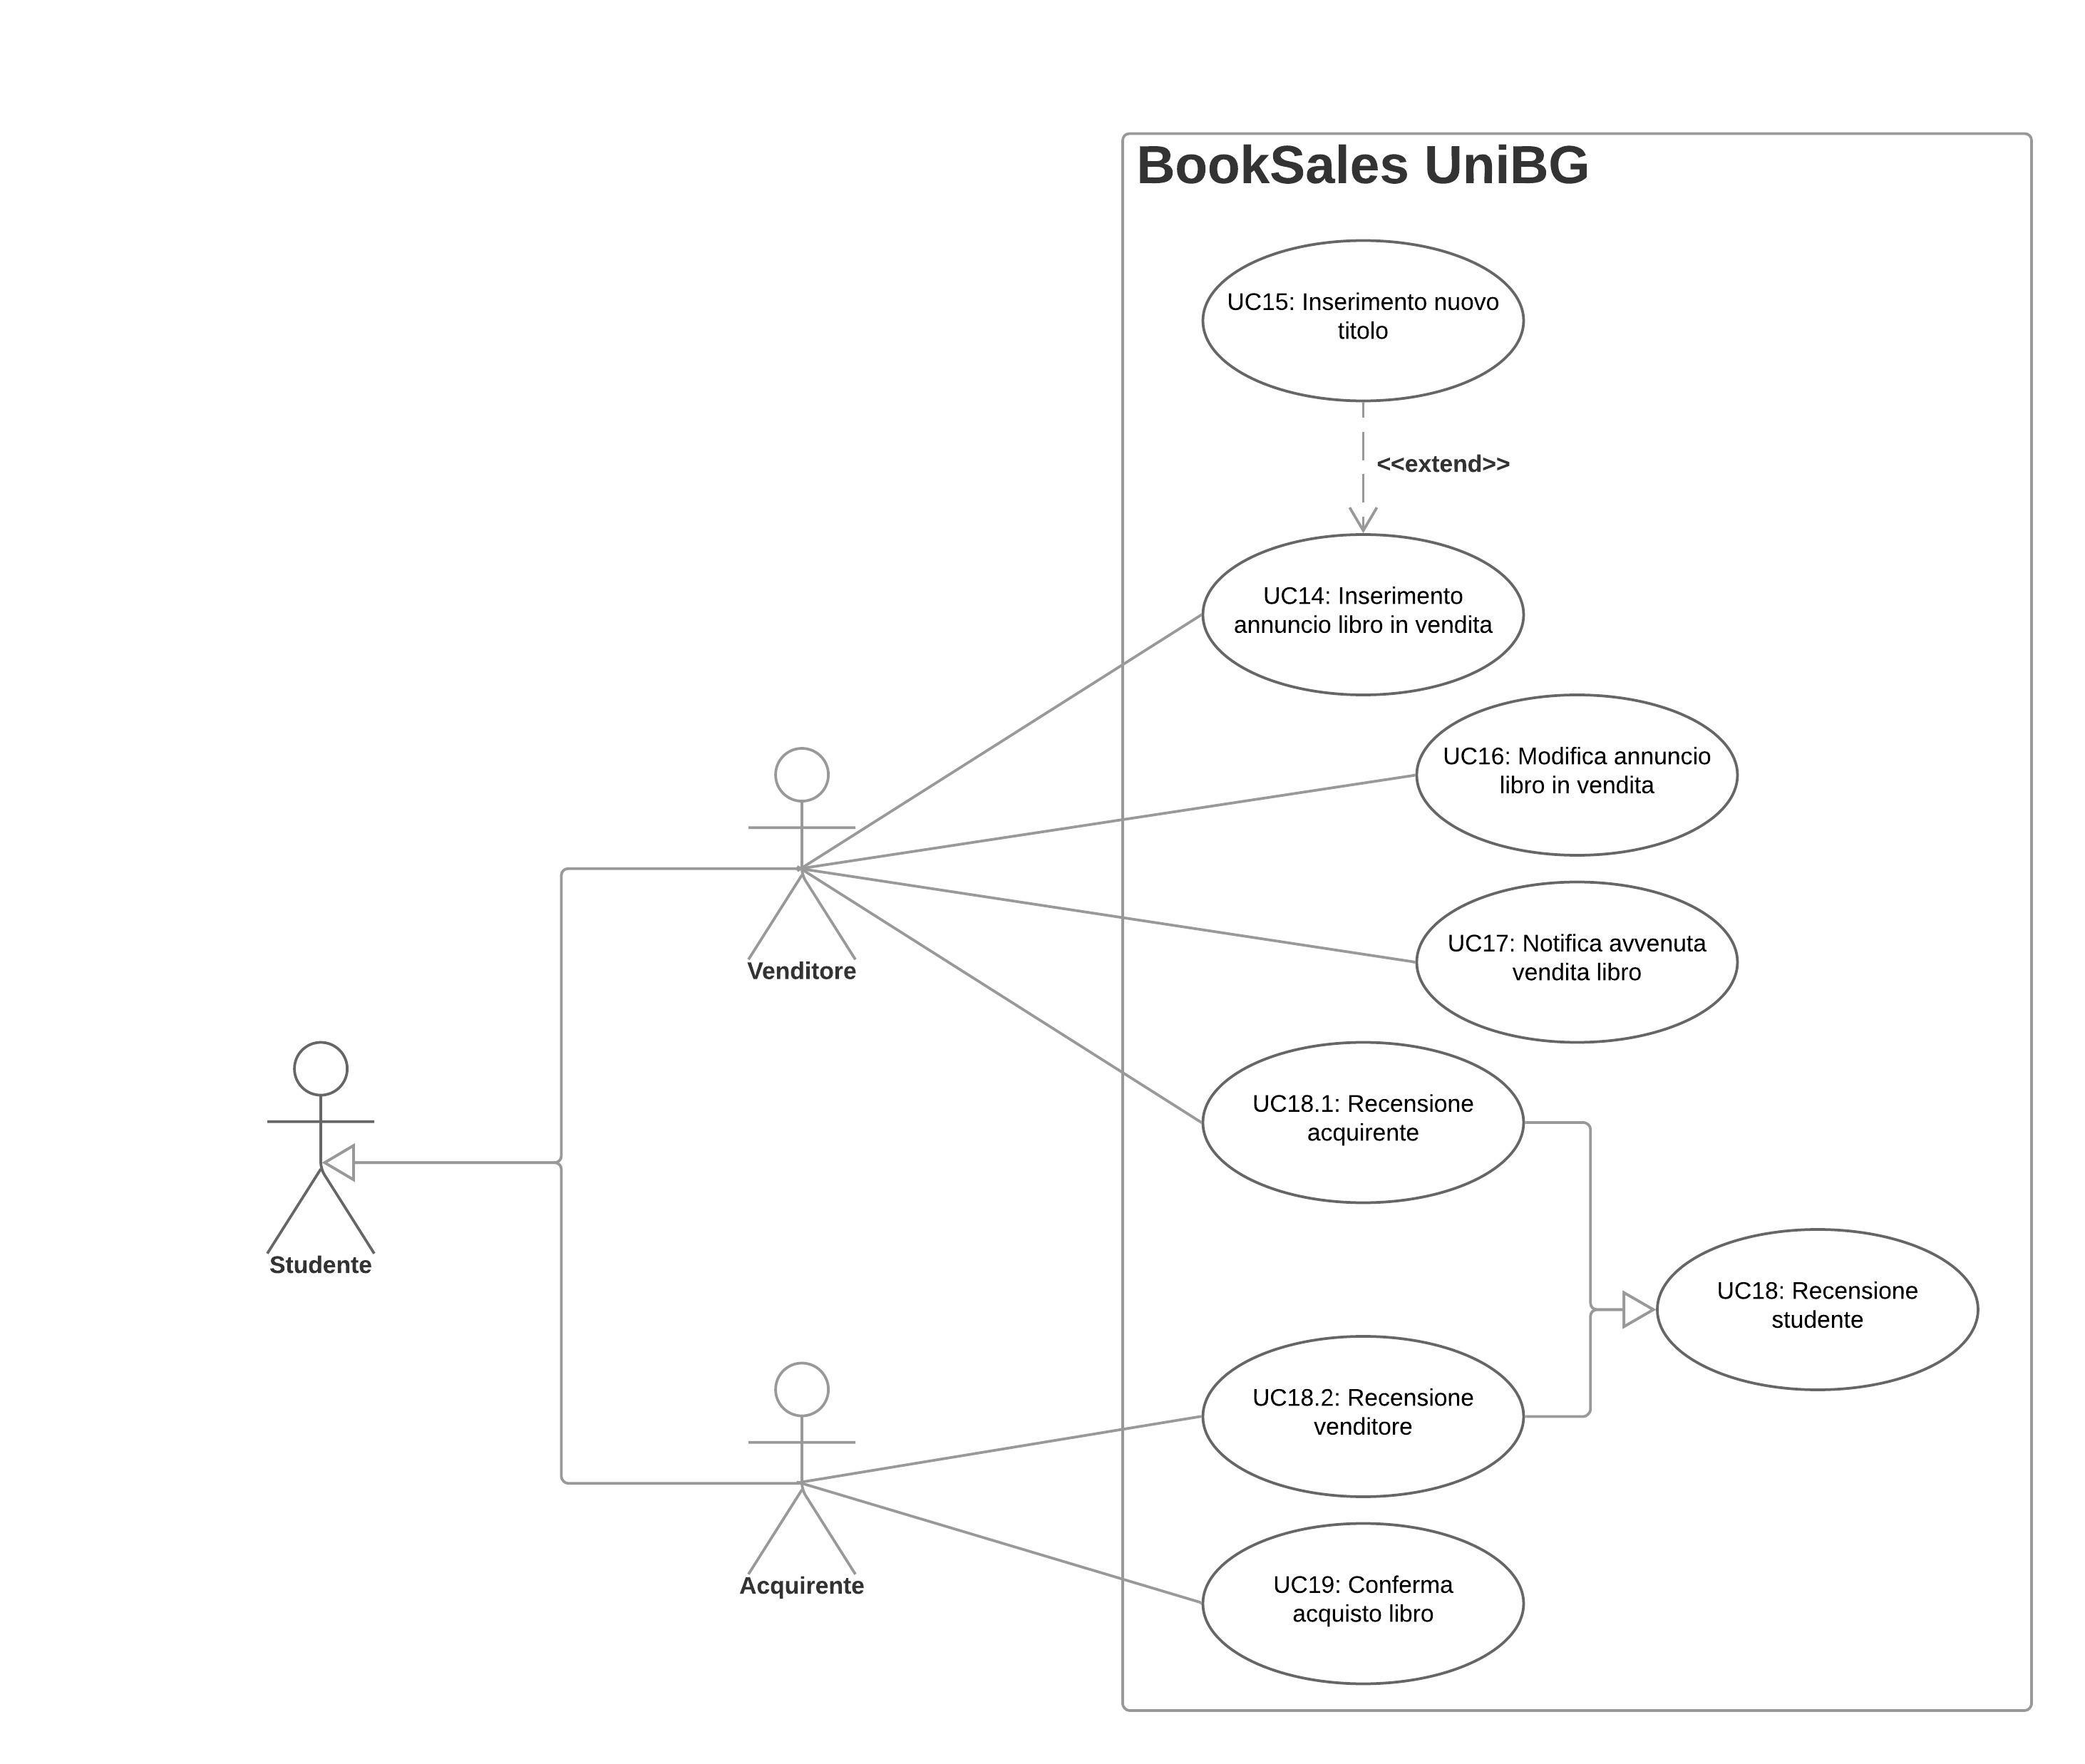
\includegraphics[height=19cm, width=17cm, keepaspectratio]{sb_uc}
		\caption{Casi d'uso per studente}
	\end{figure}

	\subsection{UC1: Registrazione studente}
	\begin{tabular}{lp{0.8\textwidth}}
		\textbf{Descrizione}&Uno studente si registra al servizio.\\
		\\
		\textbf{Requisiti coperti}&AC1\\
		\\
		\textbf{Attori coinvolti}&Studente\\
		\\
		\textbf{Precondizioni}&Lo studente che effettua la registrazione è assente dal database del sistema.\\
		\\
		\textbf{Postcondizioni}&I dati relativi al nuovo studente vengono salvati nel database.\\
		\\
		\textbf{Processo}&Di seguito è descritto il processo:
		\begin{enumerate}
			\item Lo studente accede alla pagina per la registrazione.
			\item Il sistema mostra una serie di campi da compilare:
			\begin{itemize}
				\item Username desiderato
				\item Nome e cognome
				\item Mail universitaria UniBG
				\item Corso di laurea e anno di corso
				\item Password
			\end{itemize}
			\item Lo studente compila i campi e richiede la registrazione al servizio.
			\item Il sistema verifica che tutti i campi obbligatori siano stati compilati e che rispettino le seguenti condizioni:
			\begin{itemize}
				\item La mail universitaria inserita deve terminare con il suffisso "@studenti.unibg.it" e non deve essere già stata utilizzata.
				\item La password non deve essere banale o troppo simile ai dati personali forniti.
			\end{itemize}
			\item In base al risultato delle verifiche al punto precedente il sistema si comporta in modi diversi:
			\begin{itemize}
				\item Se non tutti i campi obbligatori sono stati compilati, il sistema non effettua la registrazione ed evidenzia i campi che non sono stati compilati.
				\item Se lo username scelto risulta già utilizzato, il sistema non effettua la registrazione ed invita l'utente a scegliere un altro username.
				\item Se la mail utilizzata non rispetta le regole di cui sopra, il sistema non effettua la registrazione ed invita l'utente ad utilizzare una mail universitaria.
				\item Se tutte le condizioni sono rispettate, il sistema inserisce nel database i dati del nuovo utente e reindirizza quest'ultimo alla pagina di login.
			\end{itemize}
		\end{enumerate}
	\end{tabular}
	
	\subsection{UC2: Login studente}
	\begin{tabular}{lp{0.8\textwidth}}
		\textbf{Descrizione}&Uno studente effettua il login al sistema.\\
		\\
		\textbf{Requisiti coperti}&AC2\\
		\\
		\textbf{Attori coinvolti}&Studente\\
		\\
		\textbf{Precondizioni}&Lo studente è presente nel database del sistema.\\
		\\
		\textbf{Postcondizioni}&Lo studente può svolgere tutte le attività consentite al suo ruolo e ad un utente generico.\\
		\\
		\textbf{Processo}&Di seguito è descritto il processo:
		\begin{enumerate}
			\item Lo studente accede alla pagina per il login dedicata agli studenti.
			\item Il sistema visualizza due campi in cui inserire username e password.
			\item Lo studente inserisce username e password e richiede l'accesso.
			\item Il sistema verifica che esista uno studente registrato con lo username inserito e in caso affermativo verifica che la password inserita sia corretta.
			\item In base al risultato della ricerca precedente il sistema si può comportare in due modi:
			\begin{itemize}
				\item Se nessuno studente risulta registrato con tale username o la password è errata, il sistema impedisce l'accesso e invita l'utente ad inserire username e password corretti.
				\item Se i dati inseriti sono corretti, l'accesso viene permesso e l'utente viene reindirizzato ad una pagina di benvenuto.
			\end{itemize} 
		\end{enumerate}
	\end{tabular}

	\subsection{UC3: Logout studente}
	\begin{tabular}{lp{0.8\textwidth}}
		\textbf{Descrizione}&Uno studente effettua il logout.\\
		\\
		\textbf{Requisiti coperti}&AC3\\
		\\
		\textbf{Attori coinvolti}&Studente\\
		\\
		\textbf{Precondizioni}&Lo studente ha effettuato il login.\\
		\\
		\textbf{Postcondizioni}&La sessione dello studente corrente viene terminata.\\
		\\
		\textbf{Processo}&Di seguito è descritto il processo:
		\begin{enumerate}
			\item Lo studente clicca il link "Logout" sempre accessibile dalla barra di navigazione.
			\item Il sistema termina la sessione dello studente e reindirizza quest'ultimo alla pagina di login.
		\end{enumerate}
	\end{tabular}

	\subsection{UC4: Inserimento libro in lista "Wishlist"}
	\begin{tabular}{lp{0.8\textwidth}}
		\textbf{Descrizione}&Uno studente inserisce un libro in vendita nella propria lista "Wishlist".\\
		\\
		\textbf{Requisiti coperti}&RI3\\
		\\
		\textbf{Attori coinvolti}&Studente\\
		\\
		\textbf{Precondizioni}&Lo studente ha effettuato il login ed ha aperto la pagina relativa ad un annuncio.\\
		\\
		\textbf{Postcondizioni}&Il libro fa parte della "Wishlist" dello studente.\\
		\\
		\textbf{Processo}&Di seguito è descritto il processo:
		\begin{enumerate}
			\item Lo studente richiede l'inserimento del libro nella propria "Wishlist".
			\item Se il libro non è già presente nella wishlist, viene aggiunto e il pulsante d'aggiunta diventa verde e mostra la scritta "Added", altrimenti viene mostrato un popup che informa l'utente del fatto che il libro è già presente nella lista.
		\end{enumerate}
	\end{tabular}

	\subsection{UC5: Inserimento titolo in lista "Titoli d'interesse"}
	\begin{tabular}{lp{0.8\textwidth}}
		\textbf{Descrizione}&Uno studente inserisce un titolo nella propria lista "Titoli d'interesse".\\
		\\
		\textbf{Requisiti coperti}&RI4\\
		\\
		\textbf{Attori coinvolti}&Studente\\
		\\
		\textbf{Precondizioni}&Lo studente ha effettuato il login ed ha aperto la pagina relativa ad un titolo.\\
		\\
		\textbf{Postcondizioni}&Il titolo fa parte della lista "Titoli d'interesse" dello studente.\\
		\\
		\textbf{Processo}&Di seguito è descritto il processo:
		\begin{enumerate}
			\item Lo studente richiede l'inserimento del titolo nella propria lista "Titoli d'interesse".
			\item Se il titolo non è già presente nella lista dei titoli d'interesse, viene aggiunto e il pulsante d'aggiunta diventa verde e mostra la scritta "Added", altrimenti viene mostrato un popup che informa l'utente del fatto che il titolo è già presente nella lista.
		\end{enumerate}
	\end{tabular}

	\subsection{UC6: Accesso pagina persinale studente}
	\begin{tabular}{lp{0.8\textwidth}}
		\textbf{Descrizione}&Uno studente vuole accedere alla propria pagina personale.\\
		\\
		\textbf{Requisiti coperti}&U2.1\\
		\\
		\textbf{Attori coinvolti}&Studente\\
		\\
		\textbf{Precondizioni}&Lo studente ha effettuato il login.\\
		\\
		\textbf{Postcondizioni}&Il sistema mostra la pagina contenente le informazioni personali e i dati legati all'attività dello studente.\\
		\\
		\textbf{Processo}&Di seguito è descritto il processo:
		\begin{enumerate}
			\item Lo studente accede alla propria pagina personale tramite un link sempre visibile nella barra di navigazione, qualsiasi sia la pagina attualmente aperta.
			\item Il sistema mostra le medesime informazioni mostrate in caso di apertura della pagina personale di un altro studente, come descritto nel caso d'uso \textit{UC10}.
		\end{enumerate}
	\end{tabular}

	\subsection{UC7: Modifica impostazioni personali}
	\begin{tabular}{lp{0.8\textwidth}}
		\textbf{Descrizione}&Uno studente vuole modificare le proprie informazioni personali.\\
		\\
		\textbf{Requisiti coperti}&U3\\
		\\
		\textbf{Attori coinvolti}&Studente\\
		\\
		\textbf{Precondizioni}&Lo studente ha effettuato il login ed ha aperto la propria pagina personale.\\
		\\
		\textbf{Postcondizioni}&Il sistema permette allo studente di modificare le proprie informazioni personali e salva i cambiamenti apportati nel database.\\
		\\
		\textbf{Processo}&Di seguito è descritto il processo:
		\begin{enumerate}
			\item Lo studente accede alla propria pagina personale e richiede la modifica dei propri dati personali.
			\item Il sistema mostra una pagina contenente un elenco di campi compilabili (i campi relativi ad informazioni già fornite risultano precompilati, ma comunque modificabili) dallo studente:
			\begin{itemize}
				\item Corso di laurea e anno di corso
				\item Numero di telefono personale
				\item Indirizzo email personale
				\item Link alla pagina Facebook personale
				\item Foto profilo
			\end{itemize}
			\item Lo studente può modificare tutti i campi per poi confermare le modifiche apportate.
			\item Il sistema verifica la correttezza dei dati inseriti:
			\begin{itemize}
				\item L'indirizzo email personale, se inserito, deve contenere un simbolo '@' seguito dal nome di un dominio.
			\end{itemize}
			\item Sulla base del risultato delle verifiche effettuate al passo precedente, il sistema esegue operazioni differenti:
			\begin{itemize}
				\item Se i dati inseriti sono corretti, il sistema salva nel database i nuovi dati relativi allo studente.
				\item Se i dati inseriti non sono corretti, il sistema non effettua il salvataggio dei dati ed invita l'utente ad inserire dati corretti.
			\end{itemize}
		\end{enumerate}
	\end{tabular}

	\subsection{UC8: Modifica pagina titolo}
	\begin{tabular}{lp{0.8\textwidth}}
		\textbf{Descrizione}&Uno studente vuole modificare le proprie informazioni personali.\\
		\\
		\textbf{Requisiti coperti}&T2\\
		\\
		\textbf{Attori coinvolti}&Studente\\
		\\
		\textbf{Precondizioni}&Lo studente ha effettuato il login ed ha aperto la pagina relativa ad uno specifico titolo.\\
		\\
		\textbf{Postcondizioni}&Il sistema permette allo studente di modificare le informazioni contenute nella pagina di un titolo.\\
		\\
		\textbf{Processo}&Di seguito è descritto il processo:
		\begin{enumerate}
			\item Lo studente accede alla pagina relativa ad un titolo e ne richiede la modifica.
			\item Il sistema mostra una pagina contenente un elenco di campi compilabili (i campi relativi ad informazioni già fornite risultano precompilati, ma comunque modificabili) dallo studente:
			\begin{itemize}
				\item Immagine della copertina del libro.
				\item Descrizione degli argomenti trattati.
			\end{itemize}
			\item Il sistema salva le modifiche effettuate nel database e mostra la scritta "Modifica della pagina avvenuta con successo".
		\end{enumerate}
	\end{tabular}

	\subsection{UC9: Recensione titolo}
	\begin{tabular}{lp{0.8\textwidth}}
		\textbf{Descrizione}&Uno studente vuole recensire un titolo.\\
		\\
		\textbf{Requisiti coperti}&RE3\\
		\\
		\textbf{Attori coinvolti}&Studente\\
		\\
		\textbf{Precondizioni}&Lo studente ha effettuato il login ed ha aperto la pagina relativa ad uno specifico titolo.\\
		\\
		\textbf{Postcondizioni}&Il sistema permette allo studente di recensire il titolo e mostra la recensione sulla pagina del titolo stesso.\\
		\\
		\textbf{Processo}&Di seguito è descritto il processo:
		\begin{enumerate}
			\item Lo studente accede alla pagina relativa ad un titolo e richiede di recensire il titolo stesso.
			\item Il sistema mostra una pagina contenente un elenco di campi che devono essere compilati:
			\begin{itemize}
				\item Titolo della recensione
				\item Voto: da 0 a 5 con passo di 0.5
				\item Testo della recensione
			\end{itemize}
			\item Il sistema salva le informazioni contenute nella recensione nel database e mostra la recensione sulla pagina del titolo.
		\end{enumerate}
	\end{tabular}

	\subsection{UC10: Ricerca annuncio}
	\begin{tabular}{lp{0.8\textwidth}}
		\textbf{Descrizione}&Uno studente effettua la ricerca di un libro tra gli annunci pubblicati.\\
		\\
		\textbf{Requisiti coperti}&RI1\\
		\\
		\textbf{Attori coinvolti}&Studente\\
		\\
		\textbf{Precondizioni}&Lo studente ha effettuato il login.\\
		\\
		\textbf{Postcondizioni}&Vengono mostrati gli annunci compatibili con le keyword e i filtri inseriti dall'utente.\\
		\\
		\textbf{Processo}&Di seguito è descritto il processo:
		\begin{enumerate}
			\item Lo studente accede alla pagina relativa alla ricerca di annunci di libri in vendita.
			\item Il sistema mostra una pagina contenente una serie di campi (filtri) compilabili dall'utente per la ricerca degli annunci.
			\item Lo studente imposta i filtri sui risultati che intende ricevere. In particolare l'utente può usare i seguenti filtri:
			\begin{itemize}
				\item Titolo: può essere selezionato da una lista previa utilizzo del filtro precedente, oppure essere digitato manualmente dall'utente generico (non case-sensitive).
				\item Prezzo: possono essere scelti un prezzo massimo e/o un prezzo minimo.
				\item Condizione del libro: possono essere scelti una classe minima e/o una classe massima tra quelle introdotte nel requisito (\textit{RI1}).			
			\end{itemize}
			\item Il sistema ricerca tra gli annunci nel database i libri che risultano coerenti con i filtri imposti e mostra i risultati. In particolare per ogni risultato verranno mostrati titolo, foto, prezzo e condizione del libro, mentre la descrizione del libro e lo username del venditore vengono omessi.
			\item Lo studente può accedere ad un qualsiasi annuncio per visionare eventuali foto aggiuntive, la descrizione testuale del libro e lo username del venditore.
		\end{enumerate}
	\end{tabular}
	
	\subsection{UC11: Ricerca studente}
	\begin{tabular}{lp{0.8\textwidth}}
		\textbf{Descrizione}&Un utente effettua la ricerca di uno studente che usufruisce del servizio.\\
		\\
		\textbf{Requisiti coperti}&U1\\
		\\
		\textbf{Attori coinvolti}&Studente\\
		\\
		\textbf{Precondizioni}&Lo studente ha effettuato il login.\\
		\\
		\textbf{Postcondizioni}&Vengono mostrati gli studenti compatibili con le keyword e i filtri inseriti dall'utente.\\
		\\
		\textbf{Processo}&Di seguito è descritto il processo:
		\begin{enumerate}
			\item Lo studente accede alla pagina relativa alla ricerca di studenti iscritti al servizio.
			\item Il sistema mostra una serie di campi che possono essere compilati dallo studente per effettuare la ricerca:
			\begin{itemize}
				\item Corso di laurea ed anno di corso.
				\item Username.		
			\end{itemize}
			\item Lo studente compila i campi desiderati (corso di laurea e anno di corso hanno un valore di default) ed esegue il comando di ricerca.
			\item Il sistema ricerca tra gli studenti nel database coloro che risultano coerenti con i filtri imposti e mostra i risultati in ordine alfabetico. In particolare per ogni risultato vengono mostrati username, corso di laurea, anno di corso e una foto profilo (se questa è assente viene visualizzata un'immagine di default).
			\item Lo studente può accedere ad un qualsiasi profilo studente per visionare in dettaglio le seguenti informazioni: \textbf{DA RIVEDERE}
			\begin{itemize}
				\item Nome e cognome
				\item Indirizzo email universitario
				\item Eventuali contatti aggiuntivi quali numero di telefono, indirizzo email personale e pagina Facebook personale
				\item Numero di libri venduti
				\item Numero di libri acquistati
				\item Voto medio delle recensioni ricevute
				\item Recensioni ricevute in qualità di venditore
				\item Recensioni ricevute in qualità di acquirente
				\item Elenco dei libri in vendita
			\end{itemize}
		\end{enumerate}
	\end{tabular}
	
	\subsection{UC12: Ricerca pagina titolo}
	\begin{tabular}{lp{0.8\textwidth}}
		\textbf{Descrizione}&Uno studente effettua la ricerca della pagina relativa ad uno specifico titolo.\\
		\\
		\textbf{Requisiti coperti}&T1\\
		\\
		\textbf{Attori coinvolti}&Studente\\
		\\
		\textbf{Precondizioni}&Lo studente ha effettuato il login.\\
		\\
		\textbf{Postcondizioni}&Vengono mostrati i titoli compatibili con le keyword e i filtri inseriti dall'utente.\\
		\\
		\textbf{Processo}&Di seguito è descritto il processo:
		\begin{enumerate}
			\item Lo studente accede alla pagina relativa alla ricerca delle pagine dei titoli presenti nel sistema.
			\item Il sistema mostra una serie di campi che possono essere compilati dall'utente per effettuare la ricerca:
			\begin{itemize}
				\item Titolo: può essere selezionato da una lista previa utilizzo del filtro precedente, oppure essere digitato manualmente dall'utente generico (non case-sensitive).
				\item ISBN.			
			\end{itemize}
			\item Lo studente compila i campi (almeno uno) ed esegue il comando di ricerca.
			\item Il sistema verifica che almeno un campo sia stato compilato e sulla base del risultato di questa verifica si comporta in modo diverso:
			\begin{itemize}
				\item Se nessun campo è stato compilato, il sistema non esegue la ricerca e mostra un riquadro rosso con la scritta "Almeno un campo deve essere compilato per effettuare la ricerca".
				\item Se almeno un campo è stato compilato, procede con la ricerca.
			\end{itemize}
			\item Il sistema ricerca tra i titoli nel database quelli che risultano coerenti con i filtri imposti e mostra i risultati in ordine decrescente rispetto alla somiglianza tra le keyword utilizzate e i titoli effettivi. In particolare per ogni risultato verranno mostrati titolo e foto (se questa è assente viene visualizzata un'immagine di default).
			\item Lo studente può accedere alla pagina relativa ad un qualsiasi titolo mostrato per visionare eventuali informazioni aggiuntive, quali una descrizione (facoltativa) realizzata da altri studenti, le recensioni del titolo effettuate da altri studenti e l'elenco dei corsi per i quali il titolo è consigliato.
		\end{enumerate}
	\end{tabular}
	
	\subsection{UC13: Visualizzazione annunci consigliati}
	\begin{tabular}{lp{0.8\textwidth}}
		\textbf{Descrizione}&Uno studente visualizza un elenco di annunci consigliati per lui.\\
		\\
		\textbf{Requisiti coperti}&RI2\\
		\\
		\textbf{Attori coinvolti}&Studente\\
		\\
		\textbf{Precondizioni}&Lo studente ha effettuato il login.\\
		\\
		\textbf{Postcondizioni}&Vengono mostrati una serie di annunci consigliati per l'utente.\\
		\\
		\textbf{Processo}&Di seguito è descritto il processo:
		\begin{enumerate}
			\item Lo studente accede alla pagina "Suggested ads".
			\item Il sistema mostra una serie di annunci considerati compatibili con l'utente poiché in possesso delle seguenti caratteristiche:
			\begin{itemize}
				\item Fanno parte della Wishlist di utenti simili all'utente corrente.
				\item Fanno parte della Lista degli Interessi di utenti simili all'utente attuale.		
			\end{itemize}
		\end{enumerate}
	\end{tabular}
	
	
	\subsection{UC14: Inserimento annuncio libro in vendita}
	\begin{tabular}{lp{0.8\textwidth}}
		\textbf{Descrizione}&Uno studente nel ruolo di venditore vuole pubblicare un annuncio per la vendita di un libro.\\
		\\
		\textbf{Requisiti coperti}&I1\\
		\\
		\textbf{Attori coinvolti}&Venditore\\
		\\
		\textbf{Precondizioni}&Il venditore ha effettuato il login.\\
		\\
		\textbf{Postcondizioni}&L'annuncio viene salvato nel database.\\
		\\
		\textbf{Processo}&Di seguito è descritto il processo:
		\begin{enumerate}
			\item Lo studente accede alla pagina relativa alla pubblicazione di un annuncio.
			\item Il sistema mostra una pagina contenente un elenco di campi che devono essere compilati:
			\begin{itemize}
				\item Titolo: selezionabile da una lista dei titoli già presenti nel sistema. Se il titolo risulta assente da tale lista, la sua aggiunta è a carico del venditore (caso d'uso \textit{UCS12}).
				\item Autore/i: campo compilato automaticamente dopo la scelta del titolo.
				\item ISBN.
				\item Prezzo di vendita.
				\item Descrizione del libro.
				\item Condizioni del libro: selezione di una classe tra quelle descritte nel requisito \textit{I1}.
				\item Almeno una foto.
			\end{itemize}
			\item Lo studente compila i campi e richiede l'inserimento dell'annuncio.
			\item Il sistema verifica che tutti i campi siano stati compilati correttamente, in particolare i campi compilati manualmente dal venditore devono rispettare le seguenti regole:
			\begin{itemize}
				\item Il prezzo di vendita deve essere positivo.
				\item La descrizione deve superare i 30 caratteri.
			\end{itemize}
			\item Sulla base del risultato della verifica descritta al passo precedente, il sistema si comporta in modi diversi:
			\begin{itemize}
				\item Se tutti i campi sono stati compilati correttamente, il sistema salva l'annuncio nel database e mostra un riquadro verde con la scritta "Annuncio pubblicato con successo".
				\item Se almeno uno dei campi non è stato compilato correttamente, il sistema non salva l'annuncio e mostra un riquadro rosso con la scritta "Campi compilati in modo errato".
			\end{itemize}
		\end{enumerate}
	\end{tabular}

	\subsection{UC15: Inserimento nuovo titolo}
	\begin{tabular}{lp{0.8\textwidth}}
		\textbf{Descrizione}&Uno studente nel ruolo di venditore vuole inserire un nuovo titolo nel database del sistema.\\
		\\
		\textbf{Requisiti coperti}&I3\\
		\\
		\textbf{Attori coinvolti}&Venditore\\
		\\
		\textbf{Precondizioni}&Il venditore ha effettuato il login ed ha iniziato la procedura per l'inserimento di un nuovo annuncio, non trovando però tra i titoli selezionabili il titolo desiderato.\\
		\\
		\textbf{Postcondizioni}&Il titolo viene inserito nel database del sistema.\\
		\\
		\textbf{Processo}&Di seguito è descritto il processo:
		\begin{enumerate}
			\item Lo studente accede alla pagina relativa all'inserimento di un nuovo titolo.
			\item Il sistema mostra una pagina contenente un elenco di campi che devono essere compilati:
			\begin{itemize}
				\item Titolo: nome del libro.
				\item Autori.
				\item ISBN.
				\item Corso per il quale il libro è consigliato: selezionabile da una lista di corsi universitari.
			\end{itemize}
			\item Lo studente compila i campi e richiede l'inserimento del nuovo titolo nel database.
			\item Il sistema verifica che tutti i campi siano stati compilati correttamente, in particolare i campi compilati manualmente dal venditore devono rispettare le seguenti regole:
			\begin{itemize}
				\item Il titolo non deve essere già presente nel database.
				\item Deve essere stato citato almeno un autore.
				\item L'ISBN inserito non deve essere già presente nel database.
			\end{itemize}
			\item Sulla base del risultato della verifica descritta al passo precedente, il sistema si comporta in modi diversi:
			\begin{itemize}
				\item Se tutti i campi sono stati compilati correttamente, il sistema salva il titolo nel database, mostra un riquadro verde con la scritta "Titolo inserito correttamente, procedere con la pubblicazione dell'annuncio" e dopo 3 secondi rimanda lo studente alla pagina relativa alla pubblicazione di un annuncio.
				\item Se almeno uno dei campi non è stato compilato correttamente, il sistema non salva il titolo ed invita l'utente ad inserire dati corretti.
			\end{itemize}
		\end{enumerate}
	\end{tabular}

	\subsection{UC16: Modifica annuncio libro in vendita}
	\begin{tabular}{lp{0.8\textwidth}}
		\textbf{Descrizione}&Uno studente nel ruolo di venditore vuole modificare un annuncio da lui stesso pubblicato in passato.\\
		\\
		\textbf{Requisiti coperti}&I2\\
		\\
		\textbf{Attori coinvolti}&Venditore\\
		\\
		\textbf{Precondizioni}&Il venditore ha effettuato il login.\\
		\\
		\textbf{Postcondizioni}&Le modifiche apportate all'annuncio vengono salvate nel database.\\
		\\
		\textbf{Processo}&Di seguito è descritto il processo:
		\begin{enumerate}
			\item Lo studente accede alla pagina relativa all'annuncio che intende modificare.
			\item Il sistema verifica che lo studente sia il proprietario dell'annuncio e, in caso affermativo, oltre alle informazioni normalmente riportate mette a disposizione anche un comando "Modifica annuncio".
			\item Lo studente esegue il comando "Modifica annuncio".
			\item Il sistema mostra una pagina contenente un elenco di campi precompilati con le informazioni attuali dell'annuncio e che possono essere modificate:
			\begin{itemize}
				\item Titolo: selezionabile da una lista dei titoli già presenti nel sistema. Se il titolo risulta assente da tale lista, la sua aggiunta è a carico del venditore (caso d'uso \textit{UCS12}).
				\item Autore/i: campo compilato automaticamente dopo la scelta del titolo.
				\item ISBN.
				\item Prezzo di vendita.
				\item Descrizione del libro.
				\item Condizioni del libro: selezione di una classe tra quelle descritte nel requisito \textit{I1}.
				\item Almeno una foto.
			\end{itemize}
			\item Lo studente compila i campi e richiede la conferma della modifica dell'annuncio.
			\item Il sistema verifica che tutti i campi siano stati compilati correttamente, in particolare i campi compilati manualmente dal venditore devono rispettare le seguenti regole:
			\begin{itemize}
				\item Il prezzo di vendita deve essere positivo.
				\item La descrizione deve superare i 30 caratteri.
			\end{itemize}
		\end{enumerate}
	\end{tabular}
	
	\begin{tabular}{lp{0.8\textwidth}}
		\textbf{Processo}&\begin{enumerate}
			\setcounter{enumi}{6}
			\item Sulla base del risultato della verifica descritta al passo precedente, il sistema si comporta in modi diversi:
			\begin{itemize}
				\item Se tutti i campi sono stati compilati correttamente, il sistema salva le modifiche apportate all'annuncio nel database e notifica l'utente dell'avvenuta modifica.
				\item Se almeno uno dei campi non è stato compilato correttamente, il sistema non salva l'annuncio ed invita l'utente a compilare i campi in modo corretto.
			\end{itemize}
		\end{enumerate}
	\end{tabular}
	

	\subsection{UC17: Notifica avvenuta vendita libro}
	\begin{tabular}{lp{0.8\textwidth}}
		\textbf{Descrizione}&Uno studente nel ruolo di venditore vuole notificare al sistema l'avvenuta vendita di un libro.\\
		\\
		\textbf{Requisiti coperti}&V1\\
		\\
		\textbf{Attori coinvolti}&Venditore\\
		\\
		\textbf{Precondizioni}&Il venditore ha effettuato il login.\\
		\\
		\textbf{Postcondizioni}&Il sistema richiede allo studente indicato come acquirente del libro in oggetto di confermare l'acquisto.\\
		\\
		\textbf{Processo}&Di seguito è descritto il processo:
		\begin{enumerate}
			\item Lo studente accede alla pagina relativa all'annuncio di cui intende notificare l'avvenuta vendita.
			\item Il sistema verifica che lo studente sia il proprietario dell'annuncio e, in caso affermativo, oltre alle informazioni normalmente riportate mette a disposizione anche un comando "Notifica vendita".
			\item Lo studente esegue il comando "Notifica vendita".
			\item Il sistema mostra una pagina contenente un elenco di campi da compilare:
			\begin{itemize}
				\item Username dell'acquirente: selezionabile da un elenco di studenti iscritti al servizio.
				\item Data della cessione.
			\end{itemize}
			\item Lo studente compila i campi e sottopone i dati inseriti al controllo del sistema.
			\item Il sistema verifica che tutti i campi siano stati compilati correttamente, in particolare la data di cessione del libro non deve risultare futura rispetto alla data dell'effettiva notifica della cessione.
			\item Sulla base del risultato della verifica descritta al passo precedente, il sistema si comporta in modi diversi:
			\begin{itemize}
				\item Se tutti i campi sono stati compilati correttamente, il sistema invia una email allo studente indicato come acquirente del libro con le seguenti informazioni:
				\begin{itemize}
					\item Titolo del libro acquistato
					\item Username del venditora
					\item Prezzo d'acquisto
					\item Data dell'ipotetica cessione
				\end{itemize}
				\item Se almeno uno dei campi non è stato compilato correttamente, il sistema non invia alcuna email ed invita l'utente a compilare i campi correttamente.
			\end{itemize}
		\end{enumerate}
	\end{tabular}

	\subsection{UC18: Recensione studente}
	\subsubsection{UC18.1: Recensione acquirente}
	\begin{tabular}{lp{0.8\textwidth}}
		\textbf{Descrizione}&Uno studente nel ruolo di venditore vuole recensire l'acquirente di un proprio libro precedentemente in vendita.\\
		\\
		\textbf{Requisiti coperti}&RE2\\
		\\
		\textbf{Attori coinvolti}&Venditore\\
		\\
		\textbf{Precondizioni}&Il venditore ha effettuato il login ed è stata confermata la vendita di un libro ad uno specifico studente.\\
		\\
		\textbf{Postcondizioni}&La recensione viene pubblicata sulla pagina personale dell'acquirente.\\
		\\
		\textbf{Processo}&Di seguito è descritto il processo:
		\begin{enumerate}
			\item Lo studente accede alla pagina "Cessioni e acquisti effettuati" tramite la propria pagina personale.
			\item Il sistema mostra tutte le cessioni e gli acquisti effettuati dallo studente.
			\item Lo studente accede alla pagina relativa alla cessione d'interesse.
			\item Il sistema mostra una pagina contenente i dati relativi alla cessione:
			\begin{itemize}
				\item Titolo del libro ceduto
				\item Prezzo di cessione
				\item Data di cessione
				\item Username dell'acquirente
				\item Recensione ricevuta dall'acquirente (se presente)
				\item Recensione effettuata nei confronti dell'acquirente (se presente)
				\item Comando per la scrittura di una recensione nei confronti dell'acquirente del libro (se una recensione non è già stata effettuata)
			\end{itemize}
			\item Lo studente esegue il comando per la scrittura di una recensione.
			\item Il sistema mostra una pagina contenente dei campi da compilare:
			\begin{itemize}
				\item Titolo della recensione
				\item Voto: da 0 a 5 con passo di 0.5
				\item Testo della recensione
			\end{itemize}
			\item Il sistema verifica che tutti i campi siano stati compilati.
			\item Sulla base del risultato della verifica effettuata al passo precedente, il sistema si comporta in modo differente:
			\begin{itemize}
				\item Se i campi sono stati compilati correttamente, il sistema salva la recensione nel database e la pubblica sulla pagina personale dello studente recensito, il quale viene anche notificato tramite email della recensione ricevuta.
				\item Se i campi non sono stati compilati correttamente, il sistema non salva e non pubblica la recensione ed invita l'utente a compilare i campi in modo corretto.
			\end{itemize}
		\end{enumerate}
	\end{tabular}

	\subsubsection{UC18.2: Recensione venditore}
	\begin{tabular}{lp{0.8\textwidth}}
		\textbf{Descrizione}&Uno studente nel ruolo di acquirente vuole recensire il venditore di un libro precedentemente acquistato.\\
		\\
		\textbf{Requisiti coperti}&RE1\\
		\\
		\textbf{Attori coinvolti}&Acquirente\\
		\\
		\textbf{Precondizioni}&L'acquirente ha effettuato il login ed è stato confermato l'acquisto di un libro da uno specifico studente.\\
		\\
		\textbf{Postcondizioni}&La recensione viene pubblicata sulla pagina personale del venditore.\\
		\\
		\textbf{Processo}&Di seguito è descritto il processo:
		\begin{enumerate}
			\item Lo studente accede alla pagina "Cessioni e acquisti effettuati" tramite la propria pagina personale.
			\item Il sistema mostra tutte le cessioni e gli acquisti effettuati dallo studente.
			\item Lo studente accede alla pagina relativa all'acquisto d'interesse.
			\item Il sistema mostra una pagina contenente i dati relativi alla cessione:
			\begin{itemize}
				\item Titolo del libro acquistato
				\item Prezzo d'acquisto
				\item Data dell'acquisto
				\item Username del venditore
				\item Recensione ricevuta dal venditore (se presente)
				\item Recensione effettuata nei confronti del venditore (se presente)
				\item Comando per la scrittura di una recensione nei confronti del venditore del libro (se una recensione non è già stata effettuata)
			\end{itemize}
			\item Lo studente esegue il comando per la scrittura di una recensione.
			\item Il sistema mostra una pagina contenente dei campi da compilare:
			\begin{itemize}
				\item Titolo della recensione
				\item Voto: da 0 a 5 con passo di 0.5
				\item Testo della recensione
			\end{itemize}
			\item Il sistema verifica che tutti i campi siano stati compilati.
			\item Sulla base del risultato della verifica effettuata al passo precedente, il sistema si comporta in modo differente:
			\begin{itemize}
				\item Se i campi sono stati compilati correttamente, il sistema salva la recensione nel database e la pubblica sulla pagina personale dello studente recensito, il quale viene anche notificato tramite email della recensione ricevuta.
				\item Se i campi non sono stati compilati correttamente, il sistema non salva e non pubblica la recensione ed invita l'utente a compilare i campi in modo corretto.
			\end{itemize}
		\end{enumerate}
	\end{tabular}

	\subsection{UC19: Conferma acquisto libro}
	\begin{tabular}{lp{0.8\textwidth}}
		\textbf{Descrizione}&Uno studente nel ruolo di acquirente vuole recensire il venditore di un libro precedentemente acquistato.\\
		\\
		\textbf{Requisiti coperti}&V3\\
		\\
		\textbf{Attori coinvolti}&Acquirente\\
		\\
		\textbf{Precondizioni}&L'acquirente ha effettuato il login ed ha ricevuto una richiesta di conferma acquisto da parte di un venditore.\\
		\\
		\textbf{Postcondizioni}&L'acquisto viene confermato o negato.\\
		\\
		\textbf{Processo}&Di seguito è descritto il processo:
		\begin{enumerate}
			\item Lo studente accede alla pagina "Acquisti in attesa di conferma" tramite la propria pagina personale.
			\item Il sistema mostra tutti gli acquisti per i quali lo studente è stato indicato come acquirente.
			\item Lo studente accede alla pagina relativa all'acquisto d'interesse.
			\item Il sistema mostra una pagina contenente i dati relativi alla cessione:
			\begin{itemize}
				\item Titolo del libro acquistato
				\item Prezzo d'acquisto
				\item Data dell'acquisto
				\item Username del venditore
				\item Comando per la conferma dell'acquisto del libro
				\item Comando per la negazione dell'acquisto
			\end{itemize}
			\item Lo studente può eseguire o il comando per la conferma dell'acquisto o il comando per la negazione dello stesso.
			\item Sulla base del comando eseguito dallo studente, il sistema si comporta in modo differente:
			\begin{itemize}
				\item Se è stato eseguito il comando per la conferma dell'acquisto, il sistema esegue le seguenti operazioni:
				\begin{enumerate}
					\item Memorizza nel database le informazioni riguardanti l'avvenuto acquisto, in particolare i nomi utenti dei due studenti coinvolti, il tiolo del libro acquistato, il prezzo del libro e la data dell'acquisto.
					\item Invia una email al venditore per notificarlo dell'avvenuta conferma dell'acquisto e per invitarlo a recensire l'acquirente.
					\item Mostra una pagina in cui si invita l'acquirente a recensire il venditore con un comando "Recensisci venditore".
					\item Rimuove l'annuncio legato al libro acquistato dal database, eliminandolo quindi dalla bacheca degli annunci e da tutte le liste ("wishlist" o "titoli d'interesse") in cui era presente.
				\end{enumerate}
				\item Se è stato eseguito il comando per la negazione dell'acquisto, il sistema invia una email al venditore per notificarlo dell'errore ed invitarlo a comunicare il nome utente corretto dell'acquirente.
			\end{itemize}
		\end{enumerate}
	\end{tabular}

	\section{Class diagram}
	\begin{figure}[H]
		\centering
		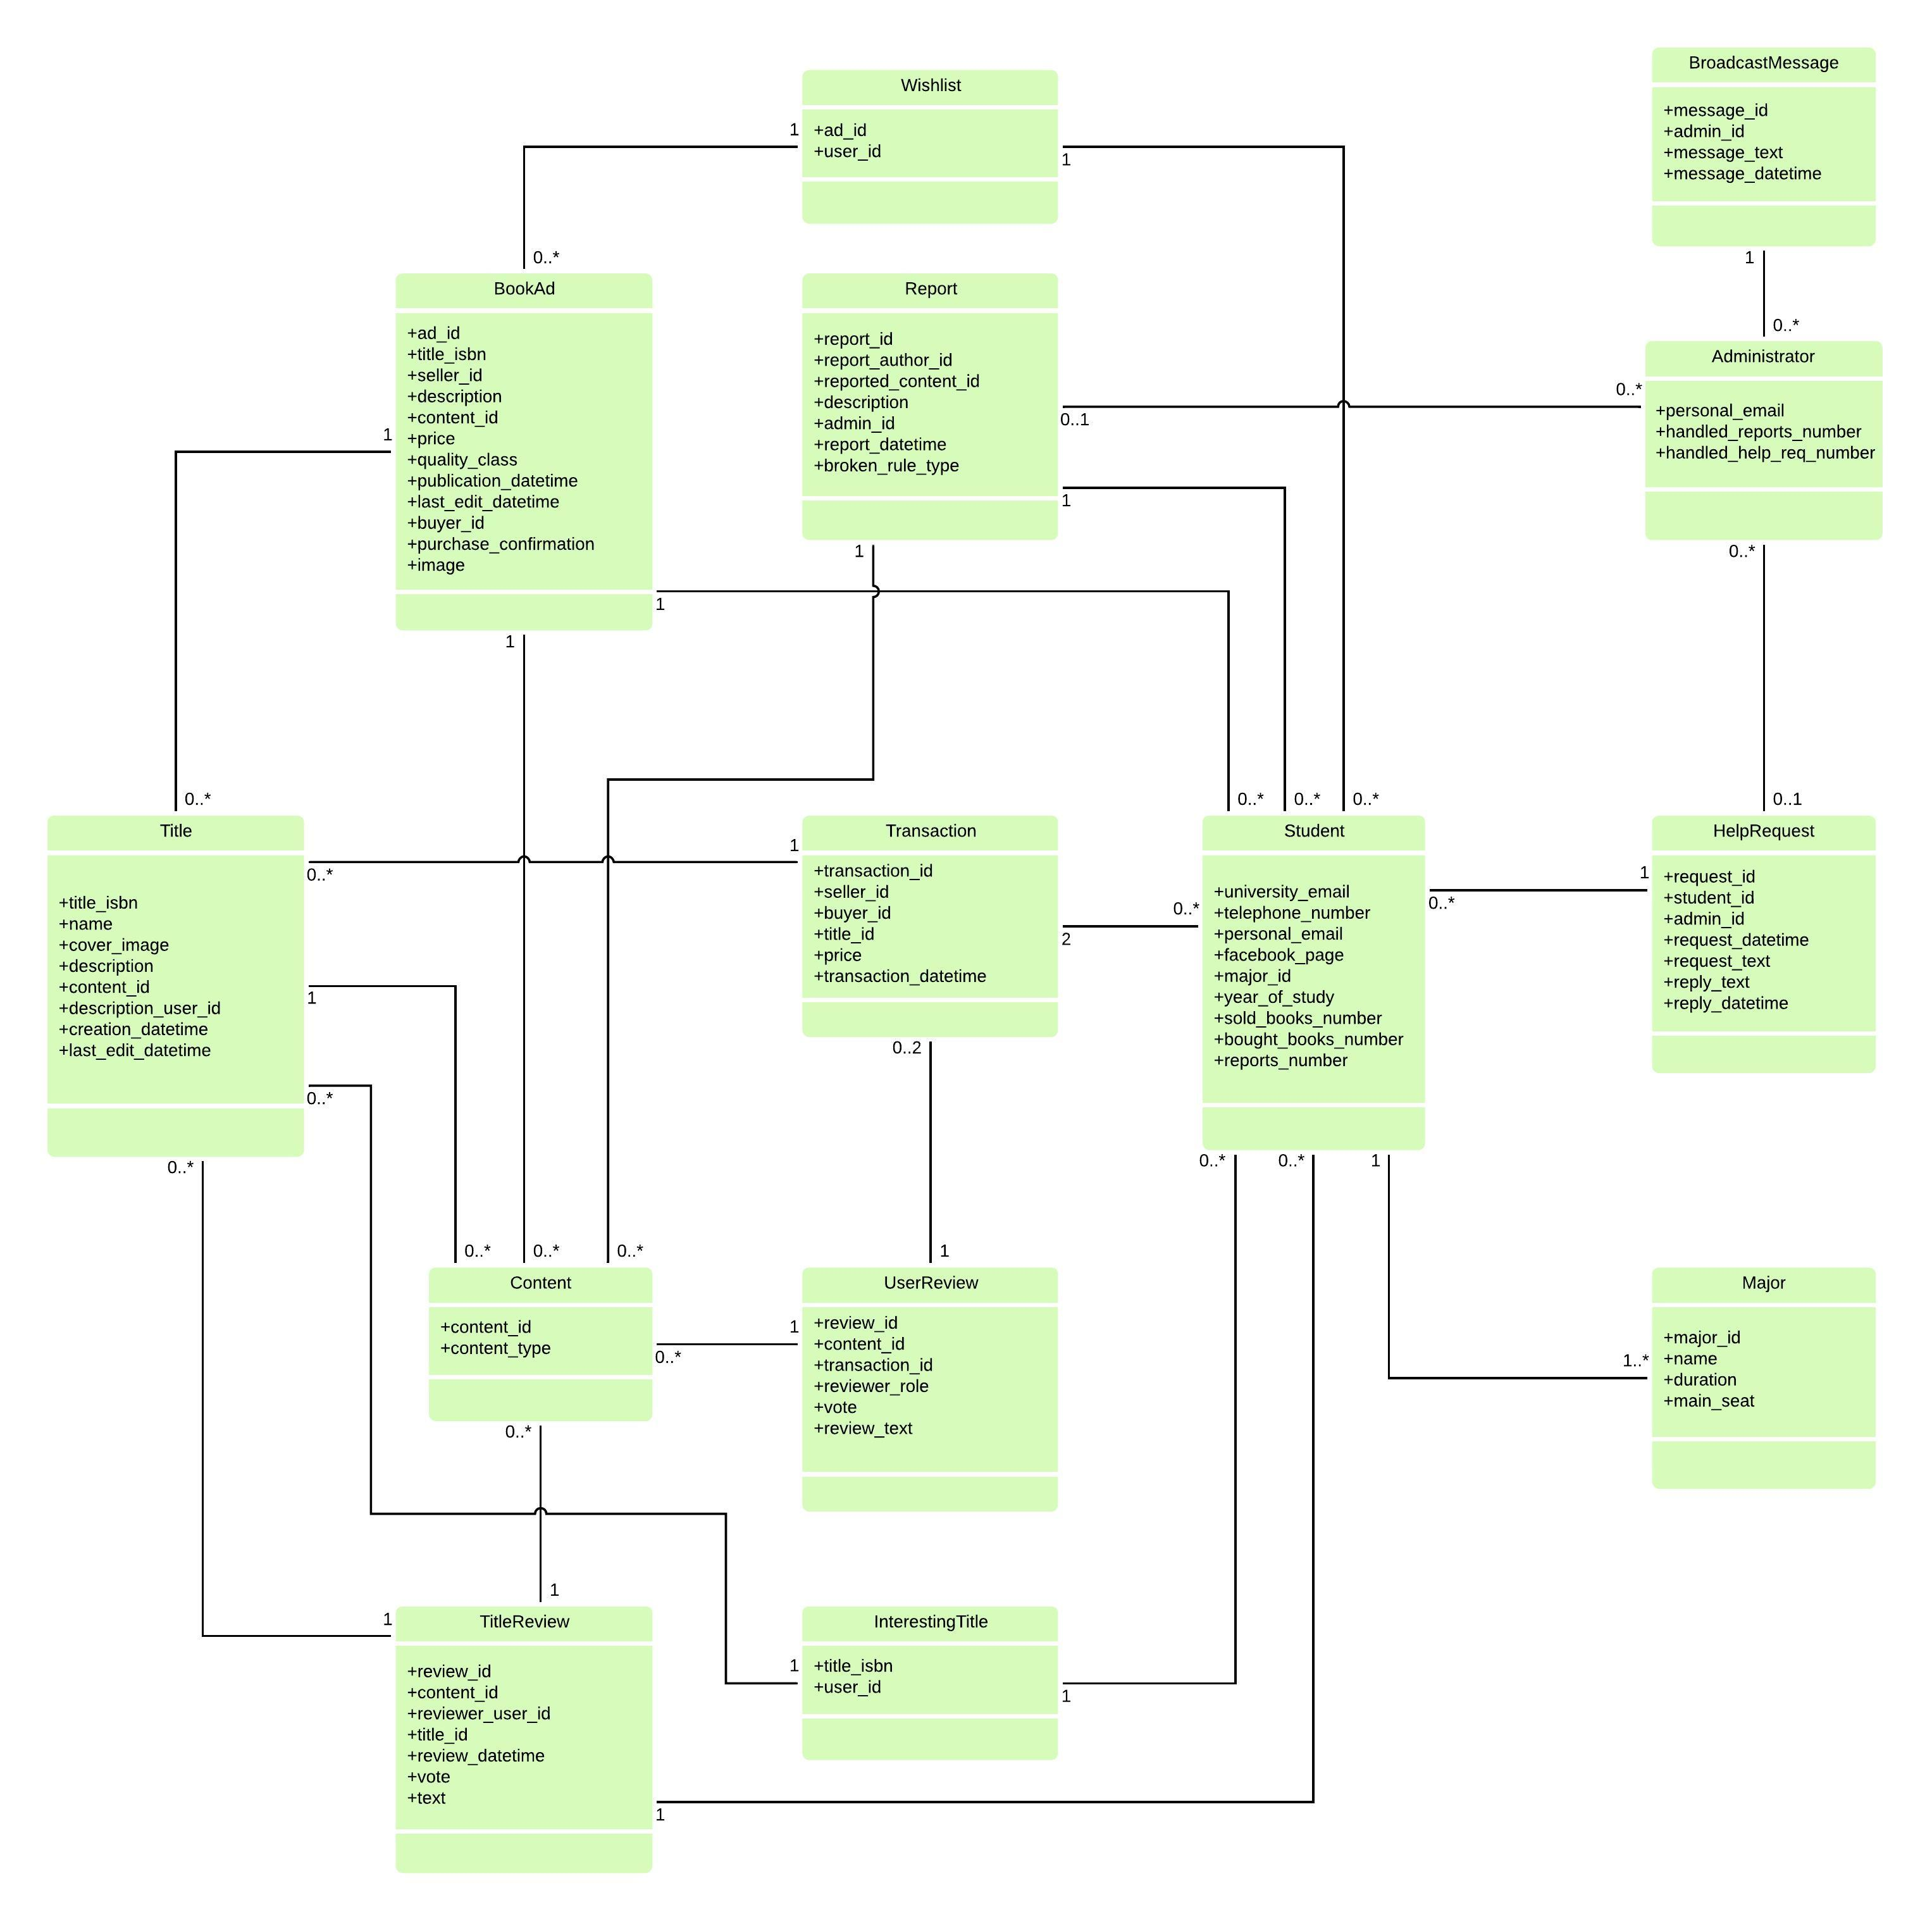
\includegraphics[height=27cm, width=17cm, keepaspectratio]{class_diagram}
		\caption{Diagramma delle classi}
	\end{figure}
	
	\section{Scelte progettuali}
	Per la realizzazione dell'applicazione sono state prese le seguenti scelte progettuali:
	\begin{itemize}
		\item Tipologia di applicazione: applicazione web, in modo da garantire un accesso semplice da qualsiasi tipo di dispositivo.
		\item Linguaggio di programmazione per l'applicazione back-end: Python 3 - framework Django 2.1, framework moderno che offre numerosi servizi di default, linguaggio ordinato e di facile lettura.
		\item Front-end: framework Bootstrap 4, per garantire una visualizzazione ottimale su dispositivi di dimensioni diverse.
		\item DBMS: Amazon RDS, DBaaS che permette di limitare responsabilità e costi legati ad una istanza reale di un DBMS. \textbf{N.B.}: la nostra implementazione utilizzerà SQLite, in quanto una simulazione del sistema progettato necessita di pochi dati e pertanto anche di un piccolo database.
		\item L'applicazione lavorerà in uno spazio messo a disposizione gratuitamente dal PaaS PythonAnywhere, specializzato nell'esecuzione di applicazioni Python.
	\end{itemize}

	\section{Toolchain}
	Le fasi di progettazione e codifica dell'applicazione verranno eseguite con l'ausilio dei seguenti tool:
	\begin{itemize}
		\item TexStudio: realizzazione della documentazione.
		\item LucidChart: realizzazione di schemi in linguaggio UML.
		\item PyCharm: IDE specifico per la programmazione in Python.
		\item Github: versioning dell'applicazione.
		\item PythonAnywhere: deployment dell'applicazione.
	\end{itemize}
	
	\section{Algoritmo: il clustering}
	Il clustering è un algoritmo di apprendimento non supervisionato (machine learning) che ha l'obiettivo di ricercare gruppi di oggetti tali che  
	gli oggetti appartenenti a un gruppo siano “simili” tra loro e differenti dagli oggetti negli altri gruppi. Dunque, in statistica, è una tecnica di 
        analisi multivariata dei dati volta al raggruppamento di elementi omogenei in un insieme di dati.\\
        Oggi le tecniche di clustering sono diffuse in diversi campi applicativi, tra i quali: il marketing, l'analisi del territorio, le assicurazioni  gli studi sismici e l'image processing.  Uno degli usi più comuni che viene fatto dei cluster, in ambito economico, 
        è proprio la segmentazione di mercato, che può essere riferita a consumatori o a categorie di prodotti con lo scopo di valutare le caratteristiche e i comportamenti dei consumatori, personalizzando l’offerta
        e incrementando dunque la quantità di prodotti venduti.
        
        		\subsection{K-means clustering}
        		Il k-means clustering è l'algoritmo di clustering più utilizzato sia in ambito accademico che in ambito industriale e funziona nel seguente modo.
        		\begin{enumerate}
        		\item Scegliere il numero di k clusters in cui raggruppare il dataset.
        		\item Selezionare casualmente k centroidi iniziali (con centroide si intende il centro geometrico di ogni cluster).
        		\item Calcolare la distanza tra ogni centroide e tutte le osservazioni.
        		\item Assegnare ognuna delle osservazione al cluster rappresentato dal centroide più vicino.
        		\item Ricalcolare la posizione dei centroidi come la posizione media delle osservazioni appartenenti al cluster che il centroide rappresenta.
        		\item Ripetere dal punto 3, finchè nessuna osservazione cambierà più il proprio cluster di appartenenza.
        		\end{enumerate}
		\textbf{Problema}: come scegliere a priori il numero di clusters?\\
		La soluzione a questo problema sta nel testare in modo iterativo più valori di k e confrontarli. 
		Per valutare il risultato viene analizzata la funzione di costo:
		\[
		J(k)=\frac{1}{k}
		\sum_{i=1}^k
		\frac{1}{n}
		\sum_{j=1}^n
		\abs{p\textsubscript{j}-c\textsubscript{i}}
		\]
		Tale funzione di costo è la media delle distanze medie delle osservazioni dal centroide del proprio cluster. E' facile notare che aumentando il numero di
		cluster diminuirà, di conseguenza, la media delle distanze delle osservazioni dai centroidi; dunque la funzione di costo è decrescente.\\
		L'\textit{elbow method} è un metodo ''grafico'' che consente di determinare il numero di cluster ideale valutando la pendenza della funzione di costo.
		Come si evince dalla figura 4, il valore ottimo di k è prossimo al punto dove la funzione di costo inizia a decrescere più lentamente.
		\begin{figure}[H]
		\centering
		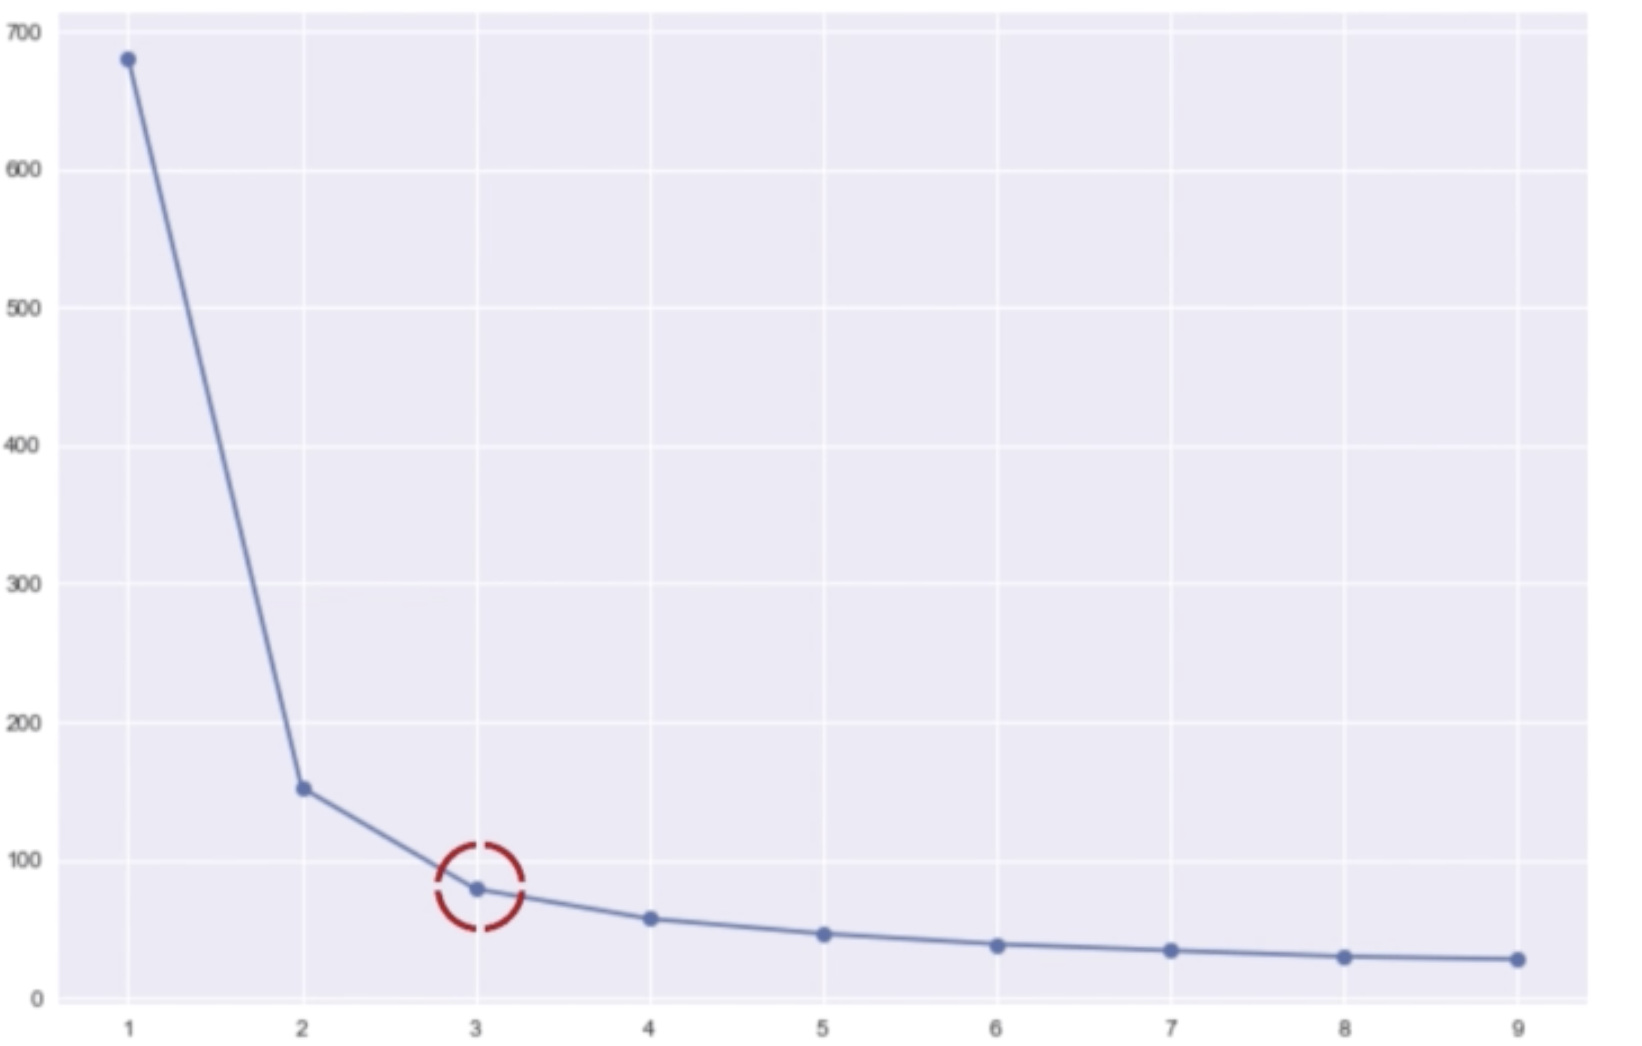
\includegraphics[scale=0.5]{elbow_method.png}
		\caption{Elbow method}
		\end{figure}
\end{document}